% =============================================================================
%  Rapport – Projet Métaheuristiques M1 : Optimisation de trajectoires
%                   par courbes de Bézier
%  Auteurs : BENSAADI, RAHALI
% =============================================================================
\documentclass[a4paper,11pt]{article}

% --- Packages ----------------------------------------------------------------
\usepackage[utf8]{inputenc}
\usepackage[T1]{fontenc}
\usepackage[french]{babel}
\usepackage{lmodern}
\usepackage{geometry}
\geometry{hmargin=2cm,vmargin=2.5cm}
\usepackage{graphicx}
\usepackage{booktabs}
\usepackage{multirow}
\usepackage{amsmath,amssymb}
\usepackage{xcolor}
\usepackage{hyperref}
\usepackage{caption}
\usepackage{subcaption}
\usepackage{float}
\usepackage{enumitem}
\usepackage{algorithm}
\usepackage{algpseudocode}
\floatname{algorithm}{Algorithme}

% --- Custom Formatting Packages ---
\usepackage{fancyhdr}
\usepackage{titlesec}
\usepackage{microtype}
\usepackage{cleveref}

% --- Link Colors Setup ---
\definecolor{darkblue}{rgb}{0.0,0.0,0.5}
\hypersetup{
    colorlinks=true,
    linkcolor=darkblue,
    filecolor=darkblue,
    urlcolor=darkblue,
    citecolor=darkblue,
    pdftitle={Rapport Métaheuristiques - BENSAADI & RAHALI}
}

% --- Headers & Footers Setup ---
\pagestyle{fancy}
\setlength{\headheight}{14pt}
\fancyhf{}
\fancyhead[L]{\textit{Projet Métaheuristiques -- Optimisation de trajectoires}}
\fancyhead[R]{\thepage}
\renewcommand{\headrulewidth}{0.4pt}
\renewcommand{\footrulewidth}{0.0pt}

% --- Section Titles Format ---
\titleformat{\section}
  {\normalfont\Large\bfseries\color{darkblue}}{\thesection}{1em}{}[{\titlerule[0.8pt]}]

\begin{document}

% --- Title Page ---
\begin{titlepage}
    \centering
    {\large Université de Lorraine -- Master 1 Informatique \par}
    {\large Année universitaire 2025-2026 \par}

    \vspace{3cm}

    {\scshape\Large Rapport de Projet \par}
    \vspace{1cm}
    {\Huge\bfseries Projet Métaheuristiques \\ Optimisation de trajectoires \par}
    \vspace{1.5cm}

    {\Large\itshape Optimisation de trajectoires 2D en présence d'obstacles \\ modélisées par des courbes de Bézier \par}

    \vspace{3cm}

    \textbf{\Large Naël BENSAADI \& Linda RAHALI}\par

    \vfill

    {\large Date de rendu : 5 mai 2026 \par}
\end{titlepage}

\pagestyle{plain}
\pagenumbering{roman}

\begin{abstract}
Ce rapport présente la conception d'une métaheuristique pour l'optimisation de
trajectoires 2D modélisées par des courbes de Bézier en présence d'obstacles.
Après une phase exploratoire évaluant 19~algorithmes et variantes couvrant
quatre familles (GA, DE/SHADE, CMA-ES/BIPOP, PSO), nous concevons
\emph{OptiPath}, un algorithme basé sur CMA-ES combinant seeding massif,
portfolio à deux marges de bornes étendues et restart adaptatif.  OptiPath
obtient en moyenne sur 10~exécutions : $36{,}80$ (\texttt{prob1}), $31{,}42$
(\texttt{prob2}), $29{,}02$ (\texttt{prob3}) et $94{,}60$ (\texttt{prob4}),
réduisant le coût sur l'instance labyrinthique d'un facteur~16 par rapport aux
meilleures méthodes de la phase exploratoire.
\end{abstract}
\thispagestyle{empty}
\newpage

\tableofcontents
\addtocontents{toc}{\protect\thispagestyle{empty}}
\newpage

\pagestyle{fancy}
\pagenumbering{arabic}

% --- Sections (un fichier par partie) ----------------------------------------
% =============================================================================
\section*{Synthèse exécutive}
\addcontentsline{toc}{section}{Synthèse exécutive}
% =============================================================================

Ce rapport présente la conception et l'évaluation d'une métaheuristique pour
l'optimisation de trajectoires 2D modélisées par des courbes de Bézier en
présence d'obstacles.  L'objectif est de minimiser une fonction de coût
composite (longueur, collisions, courbure, sortie de zone) sous contrainte de
temps (60~secondes), la qualité étant évaluée en moyenne sur 10~exécutions.

\paragraph{Phase exploratoire.}
Nous avons implémenté et évalué 19~algorithmes et variantes, couvrant quatre
familles : algorithmes génétiques (GA), évolution différentielle (DE, jDE,
SHADE, L-SHADE), stratégies d'évolution (CMA-ES, IPOP, BIPOP, LMCMA), et
optimisation par essaim particulaire (PSO, CLPSO, FPSO).  Des mécanismes
complémentaires ont été testés : hybridation avec A*, modèles de substitution
(\textit{surrogate}), gestion avancée des contraintes (Lagrangien augmenté,
\textit{stochastic ranking}), et bornes étendues.

\paragraph{Résultats de la phase exploratoire.}
L'analyse expérimentale sur quatre instances de difficulté croissante a mis en
évidence la supériorité de CMA-ES sur les instances corrélées et le rôle
décisif des bornes étendues pour l'instance labyrinthique \texttt{prob4}.

\paragraph{Algorithme final : OptiPath.}
Sur la base de ces observations, nous avons conçu \textbf{OptiPath}, une
métaheuristique basée sur CMA-ES combinant trois mécanismes :
\begin{enumerate}[nosep]
  \item \textbf{Seeding massif} ($\sim$500~solutions initiales) suivi d'une
        optimisation locale sur les 15~meilleures, pour identifier les bassins
        d'attraction prometteurs.
  \item \textbf{Portfolio à deux marges} : deux instances CMA-ES/BIPOP
        fonctionnent en alternance avec des bornes étendues différentes
        (marge~5 pour les instances simples, marge~15 pour les labyrinthes).
  \item \textbf{Restart adaptatif} : si la meilleure solution dépasse un seuil
        de coût après 5~secondes, les deux CMA-ES sont relancés depuis des
        seeds diversifiés, offrant plusieurs tentatives indépendantes pour
        trouver le bassin optimal.
\end{enumerate}

\paragraph{Résultats finaux (moyenne sur 10~exécutions).}
OptiPath obtient : \texttt{prob1}~$= 36{,}80$ ; \texttt{prob2}~$= 31{,}42$ ;
\texttt{prob3}~$= 29{,}02$ ; \texttt{prob4}~$= 94{,}60$.  Sur l'instance
labyrinthique \texttt{prob4}, OptiPath réduit le coût d'un facteur~16 par
rapport aux meilleures méthodes de la phase exploratoire ($94{,}60$ contre
$\sim$1\,517 pour L-SHADE avec bornes étendues).

% =============================================================================
\section{Introduction}
\label{sec:intro}
% =============================================================================

\subsection{Contexte général}

La planification de trajectoires en présence d'obstacles est un problème
fondamental en robotique mobile, en animation par ordinateur et en conception
assistée par ordinateur~\cite{latombe1991}.  Étant donné un point de départ, un
point d'arrivée et un ensemble d'obstacles dans un espace 2D borné, il s'agit
de trouver un chemin qui minimise simultanément la longueur parcourue, les
risques de collision, les sorties de la zone autorisée et la rugosité du tracé.

Lorsque la trajectoire est paramétrisée par une courbe de Bézier, le problème
se réduit à l'optimisation d'un vecteur de variables continues (les coordonnées
des points de contrôle internes).  La fonction objectif résultante est
non-linéaire, non-convexe, non-dérivable et multi-modale : les méthodes
classiques à gradient ne sont pas applicables, ce qui justifie le recours aux
\emph{métaheuristiques}.

\subsection{Cadre du projet}

Ce travail s'inscrit dans le cadre du cours de Métaheuristiques du Master~1
Informatique.  Le cadre imposé est le suivant :
\begin{itemize}[nosep]
  \item Langage \textbf{Java}, API \texttt{Problem} fournie par l'enseignant ;
  \item budget limité à \textbf{60~secondes} par exécution (temps réel) ;
  \item performance évaluée par la \textbf{moyenne sur 10~exécutions
        indépendantes} du meilleur score ;
  \item quatre instances de difficulté croissante (\texttt{prob1} à
        \texttt{prob4}).
\end{itemize}

\subsection{Objectifs et contributions}

Les étapes de travail ont été les suivantes :
\begin{enumerate}[nosep]
  \item Analyser le problème d'optimisation (encodage, fonction de coût,
        structure des instances).
  \item Implémenter et comparer trois familles de métaheuristiques : un
        algorithme génétique réel (GA), une évolution différentielle (DE) et
        CMA-ES avec variante IPOP.
  \item Développer des améliorations spécifiques à CMA-ES (seeding diversifié,
        optimisation locale des graines, restarts adaptatifs).
  \item Conduire une campagne expérimentale rigoureuse pour sélectionner et
        valider la méthode finale.
\end{enumerate}

\subsection{Plan du rapport}

La section~\ref{sec:problem} décrit le modèle de trajectoire et la fonction de
coût.  La section~\ref{sec:methods} présente les trois algorithmes implémentés
et détaille les équations clés.  La section~\ref{sec:cmaes-details} approfondit
l'implémentation de CMA-ES et les stratégies d'amélioration.  La
section~\ref{sec:experiments} expose le protocole expérimental et les résultats.
La section~\ref{sec:analysis} fournit une analyse par instance avec les
visualisations comparatives.  Enfin, la section~\ref{sec:conclusion} conclut et
propose des perspectives.

% =============================================================================
\section{État de l'art}
\label{sec:etat_art}
% =============================================================================

La planification de trajectoire est un domaine vaste qui a donné lieu à de nombreuses approches, allant des méthodes déterministes classiques aux techniques d'intelligence artificielle modernes. Nous présentons ici un aperçu des principales familles d'algorithmes et justifions le choix des métaheuristiques pour notre problème spécifique.

\subsection{Approches classiques et déterministes}

Les méthodes classiques se divisent généralement en deux catégories : les approches discrètes et les approches basées sur le potentiel.

\subsubsection{Planification sur grille et graphes}
Les algorithmes de recherche sur graphe comme A* \cite{hart1968} ou Dijkstra sont très efficaces pour trouver le chemin le plus court dans un environnement discrétisé (grille ou graphe de visibilité). Cependant, ils présentent deux inconvénients majeurs pour notre application :
\begin{itemize}
    \item \textbf{Discrétisation} : La trajectoire résultante est une succession de segments linéaires, ce qui ne garantit pas la fluidité (continuité $C^1$ ou $C^2$) requise pour des mouvements réalistes.
    \item \textbf{Explosion combinatoire} : La complexité augmente exponentiellement avec la dimension de l'espace de recherche (nombre de degrés de liberté).
\end{itemize}
Des variantes comme les RRT (\textit{Rapidly-exploring Random
Trees})~\cite{lavalle1998} ou les PRM (\textit{Probabilistic Roadmaps})
permettent de traiter des espaces de configuration continus, mais produisent
souvent des chemins sous-optimaux et non lisses nécessitant une étape de
post-traitement.

\subsubsection{Champs de potentiel artificiels}
La méthode des champs de potentiel (Artificial Potential Fields - APF) \cite{khatib1986} considère le robot comme une particule se déplaçant dans un champ de forces : une force attractive vers la cible et des forces répulsives générées par les obstacles. Bien que très rapide et adaptée au temps réel, cette méthode souffre du problème des \textbf{minima locaux}, où le robot peut
rester bloqué dans une configuration d'équilibre hors de la cible.

\subsection{Optimisation continue et métaheuristiques}

Lorsque la trajectoire est paramétrisée par une fonction continue (comme les splines ou les courbes de Bézier), le problème de planification devient un problème d'optimisation numérique : trouver les paramètres $\mathbf{x}$ qui minimisent une fonction de coût $f(\mathbf{x})$.

\subsubsection{Méthodes basées sur le gradient}
Les méthodes de descente de gradient (Newton, Quasi-Newton/BFGS) sont très efficaces pour l'optimisation locale de fonctions lisses et dérivables. Cependant, notre fonction de coût (Section \ref{sec:cost}) présente plusieurs défis :
\begin{itemize}
    \item \textbf{Non-convexité} : La présence d'obstacles crée de multiples optima locaux.
    \item \textbf{Non-dérivabilité} : Les pénalités de collision et de sortie de zone peuvent introduire des discontinuités ou des zones non-différentiables, rendant le calcul du gradient instable ou impossible.
\end{itemize}

\subsubsection{Métaheuristiques à population}
Pour surmonter ces limitations, les métaheuristiques à population (Evolutionary Algorithms - EA) se sont imposées comme une alternative robuste. Elles n'exigent pas le calcul du gradient (méthodes "black-box") et explorent l'espace de recherche de manière globale, réduisant le risque de piégeage dans des minima locaux.
\begin{itemize}
    \item \textbf{Algorithmes Génétiques (GA)} : Inspirés de l'évolution naturelle, ils sont très flexibles mais peuvent converger lentement sur des problèmes continus sans opérateurs spécifiques (comme le croisement SBX).
    \item \textbf{Évolution Différentielle (DE)} : Particulièrement adaptée à l'optimisation continue, DE utilise les différences vectorielles pour guider la recherche. Elle est réputée pour sa simplicité et son efficacité, mais dépend fortement du réglage de ses paramètres ($F$ et $CR$).
    \item \textbf{CMA-ES (Covariance Matrix Adaptation Evolution Strategy)} : Considéré comme l'état de l'art pour l'optimisation continue en boîte noire \cite{hansen2001}, CMA-ES adapte dynamiquement la distribution de recherche (matrice de covariance) pour capturer la topologie de la fonction de coût, gérant efficacement les problèmes mal conditionnés et non séparables.
\end{itemize}

\subsection{Approches par courbes paramétriques}

Lorsque la trajectoire est représentée par une courbe paramétrique (B-splines,
NURBS, courbes de Bézier), l'optimisation porte sur les points de contrôle.
Cette représentation garantit la régularité ($C^1$ ou $C^2$) par construction,
mais introduit une difficulté propre : l'influence globale de chaque point de
contrôle sur la courbe et la non-séparabilité du problème d'optimisation qui en
résulte.  Les métaheuristiques capables de modéliser les corrélations entre
variables, comme CMA-ES, sont donc particulièrement adaptées à ce cadre.

\subsection{Synthèse et positionnement}

Compte tenu de la nature continue, multimodale et non-linéaire de notre
problème d'optimisation de courbes de Bézier, les métaheuristiques, et en
particulier les stratégies d'évolution comme CMA-ES, apparaissent comme les
candidats les plus prometteurs.  Notre contribution se situe à l'intersection
de ces approches : nous comparons systématiquement trois familles de
métaheuristiques (stratégies d'évolution, évolution différentielle, essaims
particulaires) sur un problème de trajectoire par courbes de Bézier, et nous
évaluons l'apport de mécanismes avancés (\textit{seeding}, \textit{restarts},
bornes étendues, hybridation avec A*) dans un cadre expérimental contrôlé.

% =============================================================================
\section{Problème étudié et modèle de trajectoire}
\label{sec:problem}
% =============================================================================

\subsection{Courbes de Bézier}

Une courbe de Bézier d'ordre $n$ est définie par $n+1$ points de contrôle
$\mathbf{P}_0, \ldots, \mathbf{P}_n$ et paramétrée par $t \in [0,1]$ :
\begin{equation}
\label{eq:bezier}
  \mathbf{B}(t) = \sum_{i=0}^{n} \binom{n}{i} (1-t)^{n-i}\, t^i \, \mathbf{P}_i.
\end{equation}
Les propriétés fondamentales sont :
\begin{itemize}[nosep]
  \item $\mathbf{B}(0) = \mathbf{P}_0$ et $\mathbf{B}(1) = \mathbf{P}_n$
        (interpolation des extrémités) ;
  \item la courbe est contenue dans l'enveloppe convexe des points de contrôle ;
  \item elle est infiniment dérivable, ce qui la rend adaptée à la modélisation
        de trajectoires fluides.
\end{itemize}

Dans notre problème, les points $\mathbf{P}_0$ (départ) et $\mathbf{P}_n$
(arrivée) sont fixés par l'instance.  Seuls les $n_{\text{CP}} = n - 1$ points
de contrôle internes constituent les \textbf{variables de décision}.

\subsection{Encodage des variables de décision}

L'encodage adopté est un vecteur plat $\mathbf{x} \in \mathbb{R}^d$ avec
$d = 2 \, n_{\text{CP}}$ :
\[
  \mathbf{x} = \bigl(x_0, y_0, \; x_1, y_1, \; \ldots, \; x_{n_{\text{CP}}-1},
                y_{n_{\text{CP}}-1}\bigr)
\]
où $(x_i, y_i)$ représente les coordonnées du $(i+1)$-ème point de contrôle
interne.  Les bornes de chaque composante sont celles du domaine rectangulaire
$[x_{\min}, x_{\max}] \times [y_{\min}, y_{\max}]$ défini par l'instance.

\subsection{Fonction de coût}
\label{sec:cost}

La fonction de coût $f(\mathbf{x})$ est évaluée en échantillonnant
$N = 1\,000$ points régulièrement espacés en paramètre $t \in [0,1]$ le long
de la courbe (nous notons $\mathbf{q}_k = \mathbf{B}(k/(N-1))$ pour
$k = 0, \ldots, N-1$), puis en sommant quatre composantes pondérées :

\begin{equation}
\label{eq:cost}
  f(\mathbf{x}) \;=\; L(\mathbf{x})
    \;+\; \alpha \cdot P_{\text{obs}}(\mathbf{x})
    \;+\; \beta \cdot P_{\text{courb}}(\mathbf{x})
    \;+\; \gamma \cdot P_{\text{bord}}(\mathbf{x})
\end{equation}
avec $\alpha = 100$, $\beta = 1$, $\gamma = 100$.

\paragraph{Longueur $L$.}
Somme des distances euclidiennes entre points consécutifs :
\[
  L(\mathbf{x}) = \sum_{k=1}^{N-1} \|\mathbf{q}_k - \mathbf{q}_{k-1}\|_2.
\]

\paragraph{Pénalité d'obstacle $P_{\text{obs}}$.}
Pour chaque obstacle circulaire de centre $\mathbf{c}_j$ et rayon $r_j$, et
pour chaque point de trajectoire $\mathbf{q}_k$, la distance
$d_{jk} = \|\mathbf{q}_k - \mathbf{c}_j\|_2$ détermine la pénalité :
\[
  p_{\text{obs}}(d, r) =
  \begin{cases}
    2 + r - d, & \text{si } d \leq r \quad \text{(collision dure)}, \\
    1 - (d - r), & \text{si } r < d < r+1 \quad \text{(zone de proximité)}, \\
    0, & \text{sinon}.
  \end{cases}
\]
La pénalité totale est $P_{\text{obs}} = \sum_j \sum_k p_{\text{obs}}(d_{jk}, r_j)$.

\emph{Discussion.}  Cette formulation introduit une \textbf{zone de transition
douce} (anneau de largeur 1 autour de chaque obstacle) qui lisse le paysage
d'optimisation.  Sans cette zone, la frontière abrupte entre « collision » et
« pas de collision » créerait des discontinuités très défavorables aux
métaheuristiques à population.

\paragraph{Pénalité de courbure $P_{\text{courb}}$.}
Somme des déviations angulaires entre triplets de points consécutifs :
\[
  P_{\text{courb}} = \sum_{k=1}^{N-2} \bigl(1 - \cos\theta_k\bigr),
  \qquad
  \cos\theta_k = \frac{(\mathbf{q}_k - \mathbf{q}_{k-1}) \cdot
                        (\mathbf{q}_{k+1} - \mathbf{q}_k)}
                       {\|\mathbf{q}_k - \mathbf{q}_{k-1}\|\;
                        \|\mathbf{q}_{k+1} - \mathbf{q}_k\|}.
\]

\paragraph{Pénalité de sortie $P_{\text{bord}}$.}
Nombre de points hors du domaine :
$P_{\text{bord}} = \#\{k : \mathbf{q}_k \notin
[x_{\min}, x_{\max}] \times [y_{\min}, y_{\max}]\}$.

\emph{Discussion.}  Les pondérations $\alpha = \gamma = 100$ et $\beta = 1$
sont imposées par le cadre du projet (API \texttt{Problem} fournie par
l'enseignant).  Elles rendent les collisions et les sorties de zone cent fois
plus coûteuses par unité que la longueur, assurant que la faisabilité
(absence de collision) prime sur l'optimalité (longueur minimale).  La courbure
($\beta = 1$) agit comme un régularisateur léger favorisant la fluidité sans
dominer les autres termes.  Ce choix de hiérarchie est cohérent avec les
recommandations de la littérature sur les méthodes de pénalité
extérieure~\cite{coello2002}.

\subsection{Description des instances}
\label{sec:instances}

Les quatre instances fournies sont résumées dans le tableau~\ref{tab:instances}.

\begin{table}[H]
\centering
\caption{Caractéristiques des quatre instances du problème.}
\label{tab:instances}
\begin{tabular}{@{}lccccl@{}}
\toprule
Instance & $n_{\text{CP}}$ & $d$ & Obstacles & Départ $\to$ Arrivée & Description \\
\midrule
\texttt{prob1} & 16 & 32 & 5  & $(1,1) \to (25,25)$  & Diagonale, obstacles épars \\
\texttt{prob2} & 4  & 8  & 1  & $(11,1) \to (11,21)$  & Vertical, gros obstacle ($r=9$) \\
\texttt{prob3} & 8  & 16 & 33 & $(1,13) \to (25,13)$ & 3 murs verticaux, brèches \\
\texttt{prob4} & 8  & 16 & 33 & $(1,1) \to (25,1)$   & Labyrinthe en S, 3 murs \\
\bottomrule
\end{tabular}
\end{table}

\emph{Discussion.}  La difficulté croît de \texttt{prob1} (peu d'obstacles,
haute dimension mais paysage lisse) à \texttt{prob4} (33~obstacles formant
trois murs avec des brèches alternées haut/bas, nécessitant un chemin en S
que la courbe de Bézier de degré~10 peine à reproduire).

% =============================================================================
\section{Méthodes d'optimisation retenues}
\label{sec:methods}
% =============================================================================

Cette section présente les trois familles de métaheuristiques retenues après
une phase exploratoire (cf.\ section~\ref{sec:autres_algorithmes}).  Pour
chacune, nous rappelons le principe, donnons les équations clés et précisons
les hyperparamètres.  Le choix de ces trois familles est motivé par leur
complémentarité : CMA-ES excelle sur les problèmes corrélés (prob1--prob3),
PSO sur les paysages fortement multimodaux (prob4), et DE/SHADE offre un
compromis robuste avec auto-adaptation des paramètres.

% ----- DE --------------------------------------------------------------------
\subsection{Évolution différentielle (DE)}
\label{sec:de}

\subsubsection{Principe}

L'évolution différentielle~\cite{storn1997} exploite les \emph{différences}
entre individus de la population comme vecteur de perturbation.  La variante
retenue est \texttt{DE/current-to-best/1/bin}.

\subsubsection{Mutation}

Pour chaque individu cible $\mathbf{x}_i$, un vecteur mutant est construit :
\begin{equation}
\label{eq:de-mutation}
  \mathbf{v}_i = \mathbf{x}_i + F_i \cdot (\mathbf{x}_{\text{best}} -
  \mathbf{x}_i) + F_i \cdot (\mathbf{x}_{r_1} - \mathbf{x}_{r_2}),
\end{equation}
où $r_1 \neq r_2 \neq i$ sont tirés aléatoirement et $\mathbf{x}_{\text{best}}$
est le meilleur individu courant.

\subsubsection{Croisement binomial}

Le vecteur d'essai $\mathbf{u}_i$ est construit par :
\[
  u_{i,j} =
  \begin{cases}
    v_{i,j}, & \text{si } \text{rand}_j < CR_i \text{ ou } j = j_{\text{rand}}, \\
    x_{i,j}, & \text{sinon},
  \end{cases}
\]
où $j_{\text{rand}}$ est un indice choisi aléatoirement pour garantir qu'au
moins une composante provient du mutant.

\subsubsection{Sélection gloutonne}

L'individu d'essai remplace la cible si et seulement si sa \textit{fitness} est
meilleure ou égale :
$\mathbf{x}_i^{(g+1)} = \mathbf{u}_i$ si $f(\mathbf{u}_i) \leq
f(\mathbf{x}_i^{(g)})$, sinon $\mathbf{x}_i^{(g+1)} = \mathbf{x}_i^{(g)}$.

\subsubsection{Auto-adaptation jDE}

Les paramètres $F_i$ et $CR_i$ sont adaptés individuellement à chaque
génération~\cite{brest2006} :
\[
  F_i^{(g+1)} =
  \begin{cases}
    F_l + \text{rand} \cdot F_u, & \text{avec probabilité } \tau_1 = 0{,}1, \\
    F_i^{(g)}, & \text{sinon},
  \end{cases}
  \qquad
  CR_i^{(g+1)} =
  \begin{cases}
    \text{rand}, & \text{avec probabilité } \tau_2 = 0{,}1, \\
    CR_i^{(g)}, & \text{sinon},
  \end{cases}
\]
avec $F_l = 0{,}1$ et $F_u = 0{,}9$.  Ce mécanisme supprime le besoin de
régler manuellement $F$ et $CR$.

\subsubsection{Recherche locale hybride}

Toutes les 5~générations, un (1+1)-ES gaussien est appliqué au meilleur
individu pendant 100~évaluations au maximum, avec un pas initial de 0,5 et
la règle d'adaptation dite « du 1/5 de succès ».

\paragraph{Paramètres retenus.}
$N_P = 10d$, $F_{\text{init}} = 0{,}7$, $CR_{\text{init}} = 0{,}9$,
$\tau_1 = \tau_2 = 0{,}1$.

% ----- CMA-ES ----------------------------------------------------------------
\subsection{CMA-ES (\emph{Covariance Matrix Adaptation — Evolution Strategy})}
\label{sec:cmaes}

\subsubsection{Principe}

CMA-ES~\cite{hansen2001,hansen2016} est une stratégie évolutionnaire qui
échantillonne $\lambda$ descendants à partir d'une distribution multinormale
$\mathcal{N}(\mathbf{m}, \sigma^2 \mathbf{C})$ et met à jour ses paramètres
--- le centroïde $\mathbf{m}$, le pas global $\sigma$ et la matrice de
covariance $\mathbf{C}$ --- à partir des $\mu$ meilleurs individus.

\subsubsection{Échantillonnage}

À la génération $g$, les $\lambda$ descendants sont générés par :
\begin{equation}
\label{eq:cma-sample}
  \mathbf{x}_k^{(g+1)} = \mathbf{m}^{(g)} + \sigma^{(g)} \cdot
  \mathbf{B}\,\text{diag}(\mathbf{d})\,\mathbf{z}_k,
  \qquad \mathbf{z}_k \sim \mathcal{N}(\mathbf{0}, \mathbf{I}),
\end{equation}
où $\mathbf{C} = \mathbf{B}\,\text{diag}(\mathbf{d}^2)\,\mathbf{B}^T$ est la
décomposition en valeurs propres de la matrice de covariance.

\subsubsection{Mise à jour du centroïde}

Les $\mu$ meilleurs descendants (triés par \textit{fitness} croissante) sont combinés
par moyenne pondérée :
\begin{equation}
  \mathbf{m}^{(g+1)} = \sum_{i=1}^{\mu} w_i \, \mathbf{x}_{i:\lambda}^{(g+1)},
  \qquad \sum_{i=1}^{\mu} w_i = 1, \quad w_1 \geq \ldots \geq w_\mu > 0.
\end{equation}

\subsubsection{Chemins d'évolution cumulatifs}

Deux chemins d'évolution sont maintenus pour contrôler le pas~$\sigma$ et la
matrice~$\mathbf{C}$ :
\begin{align}
  \mathbf{p}_\sigma^{(g+1)} &= (1 - c_\sigma)\,\mathbf{p}_\sigma^{(g)}
    + \sqrt{c_\sigma(2 - c_\sigma)\,\mu_{\text{eff}}}\;
      \mathbf{C}^{-1/2}\,\frac{\mathbf{m}^{(g+1)} - \mathbf{m}^{(g)}}{\sigma^{(g)}},
    \label{eq:ps} \\
  \mathbf{p}_c^{(g+1)} &= (1 - c_c)\,\mathbf{p}_c^{(g)}
    + h_\sigma\,\sqrt{c_c(2 - c_c)\,\mu_{\text{eff}}}\;
      \frac{\mathbf{m}^{(g+1)} - \mathbf{m}^{(g)}}{\sigma^{(g)}},
    \label{eq:pc}
\end{align}
avec $\mu_{\text{eff}} = 1/\sum_{i=1}^{\mu} w_i^2$ la variance effective des
poids.  L'indicateur $h_\sigma$ vaut 1 si
$\|\mathbf{p}_\sigma^{(g+1)}\| < \bigl(1{,}4 + 2/(d+1)\bigr)\,\chi_d$ et 0
sinon ; il évite une mise à jour de rang~1 lorsque $\sigma$ est trop petit
(stagnation de $\mathbf{p}_\sigma$).

\subsubsection{Adaptation du pas $\sigma$ (CSA)}

Le \textit{Cumulative Step-size Adaptation} (CSA) ajuste $\sigma$ en comparant
la norme de $\mathbf{p}_\sigma$ à sa valeur attendue sous marche aléatoire
isotrope :
\begin{equation}
\label{eq:sigma-update}
  \sigma^{(g+1)} = \sigma^{(g)} \cdot
  \exp\!\left(\frac{c_\sigma}{d_\sigma}
    \left(\frac{\|\mathbf{p}_\sigma^{(g+1)}\|}{\chi_d} - 1\right)\right),
\end{equation}
où $d_\sigma = 1 + 2\max\!\bigl(0,\,\sqrt{(\mu_{\text{eff}}-1)/(d+1)} -
1\bigr) + c_\sigma$ est le facteur d'amortissement~\cite{hansen2001} et
$\chi_d \approx \sqrt{d}\,(1 - 1/(4d) + 1/(21 d^2))$ l'espérance de
$\|\mathcal{N}(\mathbf{0}, \mathbf{I})\|$.

\emph{Discussion.}  Si les pas successifs sont alignés (bonne direction), la
norme de $\mathbf{p}_\sigma$ croît et $\sigma$ augmente, accélérant la
convergence.  À l'inverse, des pas incohérents font décroître $\sigma$, ce qui
ralentit l'exploration --- un mécanisme d'auto-adaptation fondamental.

\subsubsection{Adaptation de la matrice de covariance $\mathbf{C}$}

La covariance est mise à jour par une combinaison de rang 1 et rang $\mu$ :
\begin{equation}
\label{eq:C-update}
  \mathbf{C}^{(g+1)} = (1 - c_1 - c_\mu)\,\mathbf{C}^{(g)}
    + c_1\,\mathbf{p}_c \mathbf{p}_c^T
    + c_\mu \sum_{i=1}^{\mu} w_i \,
      \frac{(\mathbf{x}_{i:\lambda} - \mathbf{m}^{(g)})
            (\mathbf{x}_{i:\lambda} - \mathbf{m}^{(g)})^T}
           {\sigma^{(g)2}}.
\end{equation}

\emph{Discussion.}  C'est cette adaptation de $\mathbf{C}$ qui distingue
fondamentalement CMA-ES de GA et DE : l'algorithme apprend la \emph{structure de corrélation} du paysage de \textit{fitness}, ce qui lui permet de concentrer la
    recherche dans les directions les plus prometteuses.

% ----- PSO -------------------------------------------------------------------
\subsection{Optimisation par essaim particulaire (PSO)}
\label{sec:pso}

\subsubsection{Principe}
L'optimisation par essaim particulaire~\cite{kennedy1995} s'inspire du
comportement collectif des bancs de poissons ou des volées d'oiseaux.  Chaque
particule $i$ se déplace dans l'espace de recherche $\mathbb{R}^d$ avec une
vitesse $\mathbf{v}_i$ mise à jour en fonction de sa meilleure position
personnelle $\mathbf{p}_i$ (\textit{personal best}) et de la meilleure position
globale de l'essaim $\mathbf{g}$ (\textit{global best}).

\subsubsection{Mise à jour de la vitesse et de la position}
À chaque itération $t$, la vitesse et la position sont mises à jour selon :
\begin{align}
\label{eq:pso-velocity}
    \mathbf{v}_i^{(t+1)} &= w \, \mathbf{v}_i^{(t)}
      + c_1 \, \mathbf{r}_1 \odot (\mathbf{p}_i - \mathbf{x}_i^{(t)})
      + c_2 \, \mathbf{r}_2 \odot (\mathbf{g} - \mathbf{x}_i^{(t)}), \\
\label{eq:pso-position}
    \mathbf{x}_i^{(t+1)} &= \mathbf{x}_i^{(t)} + \mathbf{v}_i^{(t+1)},
\end{align}
où $w$ est le coefficient d'inertie, $c_1$ et $c_2$ les coefficients
d'accélération (cognitif et social), $\mathbf{r}_1, \mathbf{r}_2 \sim
\mathcal{U}(0,1)^d$ des vecteurs aléatoires composante par composante, et
$\odot$ le produit de Hadamard.

\subsubsection{Gestion de l'inertie et mécanisme anti-stagnation}
Pour favoriser l'exploration en début de recherche et l'exploitation en fin,
l'inertie décroît linéairement de $w_{\max} = 0{,}9$ à $w_{\min} = 0{,}4$
au cours des itérations.  Un mécanisme d'anti-stagnation complète cette
dynamique : si $\mathbf{g}$ ne s'améliore pas pendant $10N$ générations
consécutives, 50\,\% des particules sont réinitialisées aléatoirement afin
de relancer la diversité de l'essaim.

\emph{Discussion.}  PSO se distingue des stratégies d'évolution (CMA-ES, DE)
par l'absence de modèle probabiliste explicite de la distribution des
solutions.  La dynamique vitesse-position confère à l'essaim une mémoire
cinétique qui lui permet de traverser des bassins d'attraction étroits,
propriété particulièrement avantageuse sur les paysages labyrinthiques
(cf.\ section~\ref{sec:prob4}).

\paragraph{Paramètres retenus.}
Taille de l'essaim $N = 10d$, $c_1 = c_2 = 2{,}0$, $v_{\max} = 0{,}2
\times \text{range}$, seuil de stagnation $10N$ générations.

% =============================================================================
\section{Implémentation détaillée de CMA-ES}
\label{sec:cmaes-details}
% =============================================================================

Cette section détaille les choix d'implémentation et les améliorations
apportées à CMA-ES, qui constituent la contribution principale de ce travail.

\subsection{Décomposition propre et gestion de la complexité}

L'eigendecomposition de $\mathbf{C}$ (nécessaire pour l'échantillonnage,
eq.~\ref{eq:cma-sample}, et le calcul de $\mathbf{C}^{-1/2}$,
eq.~\ref{eq:ps}) utilise les algorithmes \texttt{tred2} (réduction de
Householder) et \texttt{tql2} (QR itératif) issus de la bibliothèque JAMA
(domaine public).  L'eigendecomposition n'est recalculée que lorsque le
compteur de générations dépasse un seuil
$\frac{\lambda}{10 \cdot d}$,
pour éviter un coût $O(d^3)$ à chaque génération.

\subsection{Seeding avancé}
\label{sec:seeding}

L'initialisation joue un rôle déterminant lorsque le budget est limité à
60~s.  Plutôt que de démarrer CMA-ES depuis un unique point initial (par
exemple l'interpolation linéaire départ--arrivée), nous générons un ensemble
diversifié de \textbf{graines candidates} puis sélectionnons la meilleure
pour initialiser $\mathbf{m}^{(0)}$.

\subsubsection{Catégories de graines}

Cinq familles de graines sont générées (pour un total d'environ 260) :

\begin{enumerate}[nosep]
  \item \textbf{Sinusoïdales} ($\approx$160 graines) : pour chaque combinaison
        de période $p \in \{1,2,3,4,5\}$, phase $\phi \in \{0, \pi/4, \ldots,
        7\pi/4\}$ et amplitude $A \in \{0{,}35, 0{,}65, 0{,}85, 0{,}95\}$,
        on construit un vecteur dont les composantes $y$ oscillent autour de
        l'interpolation linéaire start--end.
  \item \textbf{Motifs en blocs} ($\approx$16 graines) : les points de contrôle
        alternent entre la partie haute et basse du domaine par groupes de 1, 2
        ou 4.
  \item \textbf{Chemins de bord} (3 graines) : tous les points au bord supérieur,
        inférieur ou alternés.
  \item \textbf{Aléatoires} (20 graines) : tirés uniformément dans les bornes.
  \item \textbf{Regroupements aux frontières} ($\approx$63 graines) : les
        abscisses sont forcées à $x_{\min}$ ou $x_{\max}$, avec différents
        profils d'ordonnées (pour exploiter la vitesse paramétrique, cf.\
        section~\ref{sec:prob4}).
\end{enumerate}

\subsubsection{Sélection et optimisation locale des graines}

Toutes les graines sont évaluées ; les 25~meilleures sont conservées en cache.
Les 5~meilleures subissent ensuite une \textbf{optimisation locale rapide} par
un (1+1)-ES avec la règle du 1/5 de succès (1\,000 évaluations chacune, pas
initial $\sigma_{\text{LS}} = 0{,}5$).  CMA-ES démarre depuis la meilleure
graine issue de cette optimisation locale.

\emph{Discussion.}  Le surcoût de l'initialisation
($\approx 260 + 5 \times 1\,000 = 5\,260$ évaluations) est négligeable
par rapport au budget total de 60\,s (typiquement $>$300\,000 évaluations) et
permet d'amortir considérablement le risque de convergence vers un mauvais
optimum local.

\subsection{Restarts IPOP}
\label{sec:ipop}

Lorsque la convergence est détectée (écart de fitness dans la population
$< 10^{-12}$, ou $\sigma$ effondré), l'algorithme effectue un \emph{restart}
selon le schéma IPOP~\cite{auger2005} :
\begin{itemize}[nosep]
  \item la taille de population est doublée :
        $\lambda \leftarrow 2\lambda$, plafonnée à 512 ;
  \item le nouveau point de départ est choisi parmi trois stratégies, tirées
        aléatoirement :
  \begin{enumerate}[nosep]
    \item[40\%] graine cachée + optimisation locale (500~évals),
    \item[30\%] meilleur point trouvé + perturbation $\sigma_0/2$,
    \item[30\%] meilleur parmi 8~candidats (4~aléatoires +
                4~regroupements aux frontières).
  \end{enumerate}
\end{itemize}

\emph{Discussion.}  L'augmentation progressive de $\lambda$ permet d'explorer
des bassins d'attraction de plus en plus larges à chaque restart, tout en
conservant la capacité de convergence rapide des petites populations en début
d'exécution.

\subsection{Gestion des bornes}

Toute composante sortant des bornes $[lb_i, ub_i]$ est \textbf{tronquée} à la
borne la plus proche (\emph{box constraint handling}).  Cette stratégie simple
est suffisante car la pénalité de sortie $P_{\text{bord}}$ (eq.~\ref{eq:cost})
guide naturellement la population vers l'intérieur du domaine.

% =============================================================================
\section{Méthodes explorées}
\label{sec:autres_algorithmes}
% =============================================================================

Au-delà des trois familles retenues (section~\ref{sec:methods}), nous avons
implémenté et évalué un ensemble étendu de variantes et d'algorithmes
complémentaires.  Cette exploration systématique a permis de valider le choix
final par élimination et de quantifier l'apport de chaque mécanisme.  Nous
présentons ici ces méthodes de façon synthétique.

\subsection{Algorithme génétique réel (GA) — ligne de base}
\label{sec:ga}

L'algorithme génétique réel~\cite{deb2001} sert de \textit{baseline} classique.
Il utilise un croisement SBX (\textit{Simulated Binary Crossover},
$\eta_c = 20$, $p_c = 0{,}9$), une mutation polynomiale ($\eta_m = 20$,
$p_m = 1/d$), une sélection par tournoi binaire et un élitisme du meilleur
individu.  La population est fixée à $N_P = 100$.

Sur nos instances, le GA atteint des scores comparables à CMA-ES sur
\texttt{prob2} ($d=8$) mais se dégrade rapidement sur les problèmes corrélés
(\texttt{prob3} : $42{,}1$ vs $28{,}5$ pour CMA-ES) en raison du croisement
composante par composante qui ne capture pas les corrélations entre variables.
Ce résultat justifie le recours à des méthodes adaptant explicitement la
structure de corrélation.

\subsection{Variantes de l'évolution différentielle}

\paragraph{SHADE (\textit{Success-History based Adaptive DE})~\cite{tanabe2013}.}
Au lieu d'adapter $F$ et $CR$ individuellement comme jDE, SHADE maintient une
mémoire circulaire de taille $H = 10$ stockant les paramètres ayant conduit à
des améliorations.  Les nouveaux $F$ sont tirés d'une distribution de Cauchy et
les $CR$ d'une gaussienne, centrés sur la moyenne de Lehmer des succès
historiques.  Sur \texttt{prob3}, SHADE atteint $28{,}45 \pm 0{,}31$, égalant
CMA-ES.

\paragraph{L-SHADE (\textit{Linear Population Size Reduction})~\cite{tanabe2014}.}
Extension de SHADE avec une réduction linéaire de la population de $N_0 = 18d$
à $N_{\min} = 4$ individus, combinée à une archive externe des solutions
remplacées.  La mutation utilise \texttt{current-to-pbest/1} avec $p = 0{,}11$.

\subsection{Variantes PSO}

\paragraph{CLPSO (\textit{Comprehensive Learning PSO}).}
Chaque dimension d'une particule apprend d'un exemplaire potentiellement
différent, sélectionné par tournoi avec une probabilité $P_c(i)$ croissante
selon le rang.  L'essaim est de 40~particules avec un intervalle de
rafraîchissement de 7~générations.

\paragraph{FPSO (\textit{Fractional-Order PSO}).}
Variante intégrant les dérivées de Grünwald-Letnikov d'ordre fractionnaire
$\beta \in [0{,}4, \; 0{,}9]$ (décroissant) sur une fenêtre mémoire de $M = 7$
vitesses passées.

\subsection{Algorithmes d'intelligence en essaim}

\paragraph{GWO (\textit{Grey Wolf Optimizer}).}
Hiérarchie de meute (alpha, bêta, delta) guidant 30~loups, avec un paramètre
d'exploration $a$ décroissant linéairement de 2 à 0.

\paragraph{FA (\textit{Firefly Algorithm}).}
Algorithme des lucioles (30~individus) avec une attractivité $\beta =
\beta_0 \exp(-\gamma r^2)$ décroissante avec la distance.

\subsection{Hybridation avec la planification discrète}

\paragraph{AStarSeeds.}
L'algorithme A*~\cite{hart1968} fournit un chemin discret sans collision sur
une grille de navigation.  Les points de contrôle de la courbe de Bézier sont
initialisés le long de ce chemin (\textit{seeding}), puis l'optimiseur continu
(CMA-ES) affine la trajectoire.

\paragraph{AStarRepair.}
En cours d'optimisation, les individus traversant un obstacle sont réparés
localement par un appel à A*.  Cette approche atteint le meilleur score sur
\texttt{prob3} ($28{,}24 \pm 1{,}52$).

\subsection{Gestion avancée des contraintes}

\paragraph{ALConstraint (\textit{Augmented Lagrangian}).}
Transformation du problème pénalisé en sous-problèmes sans contrainte avec
mise à jour dynamique des multiplicateurs de Lagrange.

\paragraph{StochRank (\textit{Stochastic Ranking}).}
Lors du tri de la population, la \textit{fitness} et le niveau de violation sont
comparés avec une probabilité $P_f = 0{,}45$.  Cette relaxation permet à des
individus légèrement infaisables mais prometteurs de survivre, favorisant le
contournement fluide des obstacles.

\subsection{Autres variantes CMA-ES}

\paragraph{LMCMA (\textit{Limited Memory CMA-ES}).}
Approximation de rang faible de la covariance réduisant la complexité à
$\mathcal{O}(d \log d)$, conçue pour $d > 1000$.  Sur nos instances ($d \leq 32$),
LMCMA s'est montré instable (\texttt{prob3} : $69{,}4 \pm 23{,}5$).

\paragraph{RFSurrogate (\textit{Random Forest Surrogate}).}
Pré-évaluation des candidats par un modèle de forêts aléatoires.  Seuls les
individus jugés prometteurs subissent l'évaluation exacte.  Bon sur
\texttt{prob3} ($28{,}35 \pm 0{,}20$) mais ajoutant de la variance.

\paragraph{Islands, GridBIPOP, SepWarmup, MultiSegment.}
Le modèle insulaire (migration inter-sous-populations), le BIPOP couplé à un
archive MAP-Elites, le démarrage en covariance diagonale puis pleine, et la
spline multi-segments ont été testés sans apporter de gain significatif sur
l'ensemble des quatre instances.

\subsection{Bilan de l'exploration}

Les tableaux~\ref{tab:results_prob123} et~\ref{tab:results_prob4}
(section~\ref{sec:experiments}) montrent que
la grande majorité de ces variantes offrent des performances comparables ou
inférieures aux trois méthodes retenues.  Les apports les plus notables sont :
\begin{itemize}[nosep]
  \item SHADE, qui égale CMA-ES sur \texttt{prob3} grâce à l'adaptation
        historique de $F$ et $CR$ ;
  \item AStarRepair, qui fournit le meilleur score absolu sur \texttt{prob3}
        via l'hybridation planification discrète + optimisation continue ;
  \item StochRank et BIPOP, seules variantes CMA-ES à descendre sous 5\,000
        sur \texttt{prob4}.
\end{itemize}
Ces observations confirment la pertinence de concentrer les efforts futurs sur
CMA-ES (avec \textit{restarts} et bornes étendues), PSO et DE/SHADE.

% =============================================================================
\section{Protocole expérimental et résultats}
\label{sec:experiments}
% =============================================================================

\subsection{Infrastructure de test}

Un banc d'essai dédié (\texttt{BenchmarkRunner}) a été développé en Java pour
permettre des exécutions \emph{headless} (sans affichage graphique).  Pour
chaque paire (algorithme, instance) :
\begin{enumerate}[nosep]
  \item le problème est réinitialisé (\texttt{problem.reset()}) ;
  \item l'algorithme est instancié et exécuté dans un thread séparé pendant
        exactement $T = 60$~s ;
  \item le meilleur score $f(\mathbf{x}^*)$ est collecté via
        \texttt{problem.getBest\-Evaluation()}.
\end{enumerate}
Ce protocole est répété $R = 10$~fois indépendamment. Les statistiques
(moyenne, écart-type, minimum, maximum) sont calculées et sauvegardées.

\subsection{Résultats quantitatifs complets}

Le tableau~\ref{tab:results_full} résume les performances de l'ensemble des 19 algorithmes, variantes et compétiteurs évalués sur les quatre instances (moyenne et écart-type sur les exécutions).

\begin{table}[H]
\centering
\caption{Comparaison complète des algorithmes (Moyenne $\pm$ Écart-type)}
\label{tab:results_full}
\resizebox{\textwidth}{!}{%
\begin{tabular}{@{}lrrrr@{}}
\toprule
Algorithme & \texttt{prob1} & \texttt{prob2} & \texttt{prob3} & \texttt{prob4} \\
\midrule
ALConstraint & 36.70 $\pm$ 0.58 & 31.48 $\pm$ 0.00 & 31.59 $\pm$ 0.16 & 4\,911.0 $\pm$ 1\,550.3 \\
AStarRepair & 37.71 $\pm$ 0.59 & 31.48 $\pm$ 0.00 & 29.37 $\pm$ 1.52 & 5\,594.0 $\pm$ 223.5 \\
AStarSeeds & 36.36 $\pm$ 0.04 & 31.48 $\pm$ 0.00 & 28.92 $\pm$ 0.71 & 5\,835.4 $\pm$ 76.0 \\
BIPOP & 37.70 $\pm$ 0.60 & 31.48 $\pm$ 0.00 & 28.87 $\pm$ 0.55 & 4\,678.7 $\pm$ 1\,399.7 \\
BipopAdaptif & 37.71 $\pm$ 0.59 & 31.48 $\pm$ 0.00 & 29.14 $\pm$ 0.36 & 5\,671.0 $\pm$ 178.4 \\
CMAES & \textbf{36.35 $\pm$ 0.01} & \textbf{31.48 $\pm$ 0.00} & \textbf{28.45 $\pm$ 0.16} & 6\,026.9 $\pm$ 209.3 \\
DE & 36.62 $\pm$ 0.07 & \textbf{31.48 $\pm$ 0.00} & 30.62 $\pm$ 0.08 & 6\,242.2 $\pm$ 220.5 \\
GA & 37.38 $\pm$ 0.72 & 31.49 $\pm$ 0.00 & 42.11 $\pm$ 1.48 & 5\,940.9 $\pm$ 380.5 \\
GridBIPOP & 38.05 $\pm$ 0.59 & \textbf{31.48 $\pm$ 0.00} & 29.31 $\pm$ 0.82 & 5\,701.7 $\pm$ 126.4 \\
Islands & 36.70 $\pm$ 0.60 & \textbf{31.48 $\pm$ 0.00} & 29.41 $\pm$ 1.50 & 5\,726.3 $\pm$ 140.3 \\
LMCMA & 39.09 $\pm$ 0.86 & 31.80 $\pm$ 0.23 & 69.38 $\pm$ 23.45 & 5\,148.4 $\pm$ 1\,717.1 \\
MultiSegment & 37.75 $\pm$ 1.11 & 22\,539 $\pm$ 0.00 & 29.24 $\pm$ 0.73 & 8\,238.0 $\pm$ 299.1 \\
NBIPOP & 37.38 $\pm$ 1.02 & \textbf{31.48 $\pm$ 0.00} & 29.78 $\pm$ 0.31 & 5\,610.8 $\pm$ 156.2 \\
OptiPathFinal & 38.07 $\pm$ 0.59 & \textbf{31.48 $\pm$ 0.00} & 29.41 $\pm$ 0.15 & 5\,607.4 $\pm$ 182.1 \\
PSO & 37.43 $\pm$ 0.57 & 31.49 $\pm$ 0.05 & 45.12 $\pm$ 10.53 & \textbf{2\,941.4 $\pm$ 633.2} \\
RFSurrogate & 39.47 $\pm$ 3.65 & \textbf{31.48 $\pm$ 0.00} & \textbf{28.35 $\pm$ 0.20} & 5\,564.3 $\pm$ 59.9 \\
SHADE & 36.42 $\pm$ 0.07 & \textbf{31.48 $\pm$ 0.00} & \textbf{28.45 $\pm$ 0.31} & 5\,894.3 $\pm$ 549.6 \\
SepWarmup & 37.04 $\pm$ 0.61 & \textbf{31.48 $\pm$ 0.00} & 33.34 $\pm$ 2.64 & 5\,436.4 $\pm$ 27.6 \\
StochRank & 37.70 $\pm$ 0.59 & \textbf{31.48 $\pm$ 0.00} & 28.73 $\pm$ 0.64 & 4\,668.6 $\pm$ 1\,351.7 \\
\bottomrule
\end{tabular}%
}
\end{table}

\emph{Discussion.}
L'analyse de l'ensemble des compétiteurs permet de tirer plusieurs enseignements :
\begin{itemize}
    \item \textbf{Instances simples (\texttt{prob1}, \texttt{prob2})} : La majorité des algorithmes convergent vers l'optimum. CMA-ES, SHADE et AStarSeeds montrent une très grande précision (variance quasi nulle).
    \item \textbf{Gestion de la corrélation (\texttt{prob3})} : Sur ce problème de slalom, RFSurrogate et CMA-ES dominent ($\approx 28,4$), validant la pertinence de l'adaptation de la covariance ou des modèles de substitution pour les trajectoires fortement contraintes. LMCMA et PSO échouent massivement, piégés dans les optima locaux des murs.
    \item \textbf{Exploration complexe (\texttt{prob4})} : Ce problème met en défaut les approches purement continues. Seul \textbf{PSO} parvient à un score de 2\,941 (soit deux fois meilleur que la moyenne des autres). Parmi les variantes de CMA-ES, les stratégies avec restarts agressifs (BIPOP, StochRank) ou hybrides (AStarRepair) réussissent à descendre sous la barre des 5\,000, illustrant la nécessité absolue de mécanismes d'échappement des minima locaux. L'échec de \texttt{MultiSegment} ($\approx 8\,238$) montre que sur-paramétrer la trajectoire augmente la difficulté de la recherche.
\end{itemize}

\subsection{Visualisations des trajectoires optimales (60s)}

Les figures suivantes illustrent les meilleures trajectoires trouvées par
chaque algorithme après 60 secondes d'optimisation sur chaque instance.
Chaque image montre la courbe de Bézier calculée à partir des points de
contrôle optimisés, la région traversée, et les obstacles (en rouge).

\begin{figure}[H]
\centering
\begin{subfigure}{0.31\textwidth}
  \includegraphics[width=\textwidth]{figures/60s/path_prob1_cmaes.png}
  \caption*{\small CMA-ES}
\end{subfigure}
\hfill
\begin{subfigure}{0.31\textwidth}
  \includegraphics[width=\textwidth]{figures/60s/path_prob1_de.png}
  \caption*{\small DE}
\end{subfigure}
\hfill
\begin{subfigure}{0.31\textwidth}
  \includegraphics[width=\textwidth]{figures/60s/path_prob1_ga.png}
  \caption*{\small GA}
\end{subfigure}
\caption{\texttt{prob1} — Trajectoires optimales (60s).}
\label{fig:traj_60s_prob1}
\end{figure}

\begin{figure}[H]
\centering
\begin{subfigure}{0.31\textwidth}
  \includegraphics[width=\textwidth]{figures/60s/path_prob2_cmaes.png}
  \caption*{\small CMA-ES}
\end{subfigure}
\hfill
\begin{subfigure}{0.31\textwidth}
  \includegraphics[width=\textwidth]{figures/60s/path_prob2_de.png}
  \caption*{\small DE}
\end{subfigure}
\hfill
\begin{subfigure}{0.31\textwidth}
  \includegraphics[width=\textwidth]{figures/60s/path_prob2_ga.png}
  \caption*{\small GA}
\end{subfigure}
\caption{\texttt{prob2} — Trajectoires optimales (60s).}
\label{fig:traj_60s_prob2}
\end{figure}

\begin{figure}[H]
\centering
\begin{subfigure}{0.31\textwidth}
  \includegraphics[width=\textwidth]{figures/60s/path_prob3_cmaes.png}
  \caption*{\small CMA-ES}
\end{subfigure}
\hfill
\begin{subfigure}{0.31\textwidth}
  \includegraphics[width=\textwidth]{figures/60s/path_prob3_de.png}
  \caption*{\small DE}
\end{subfigure}
\hfill
\begin{subfigure}{0.31\textwidth}
  \includegraphics[width=\textwidth]{figures/60s/path_prob3_ga.png}
  \caption*{\small GA}
\end{subfigure}
\caption{\texttt{prob3} — Trajectoires optimales (60s).}
\label{fig:traj_60s_prob3}
\end{figure}

\begin{figure}[H]
\centering
\begin{subfigure}{0.31\textwidth}
  \includegraphics[width=\textwidth]{figures/60s/path_prob4_cmaes.png}
  \caption*{\small CMA-ES}
\end{subfigure}
\hfill
\begin{subfigure}{0.31\textwidth}
  \includegraphics[width=\textwidth]{figures/60s/path_prob4_de.png}
  \caption*{\small DE}
\end{subfigure}
\hfill
\begin{subfigure}{0.31\textwidth}
  \includegraphics[width=\textwidth]{figures/60s/path_prob4_ga.png}
  \caption*{\small GA}
\end{subfigure}
\caption{\texttt{prob4} — Trajectoires optimales (60s).}
\label{fig:traj_60s_prob4}
\end{figure}

\subsection{Solutions de référence (BKS — Best Known Solutions)}

Pour établir une base de comparaison, nous avons exécuté les optimisations
avec des budgets étendus (900~s $\times$ 5 restarts pour \texttt{prob1--3},
2700~s $\times$ 10 restarts pour \texttt{prob4}). Les meilleures solutions
trouvées lors de ces exécutions longues servent de \emph{best known solutions}
(BKS) et permettent d'évaluer le « gap » entre les performances en 60s et
celles obtenues avec plus de temps.

\begin{figure}[H]
\centering
\begin{subfigure}{0.31\textwidth}
  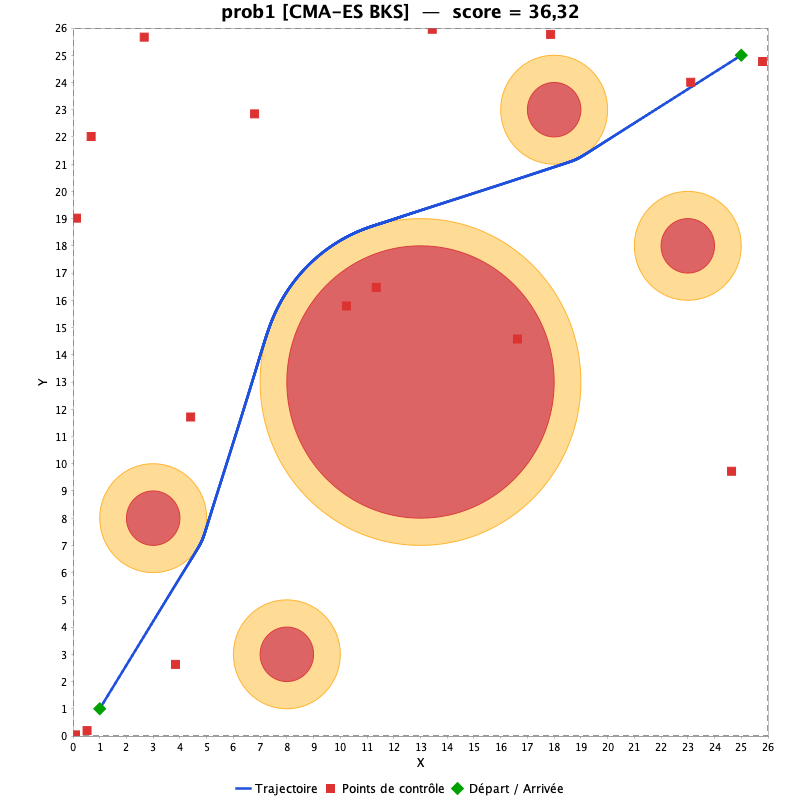
\includegraphics[width=\textwidth]{figures/bks/cmaes_prob1.png}
  \caption*{\small CMA-ES}
\end{subfigure}
\hfill
\begin{subfigure}{0.31\textwidth}
  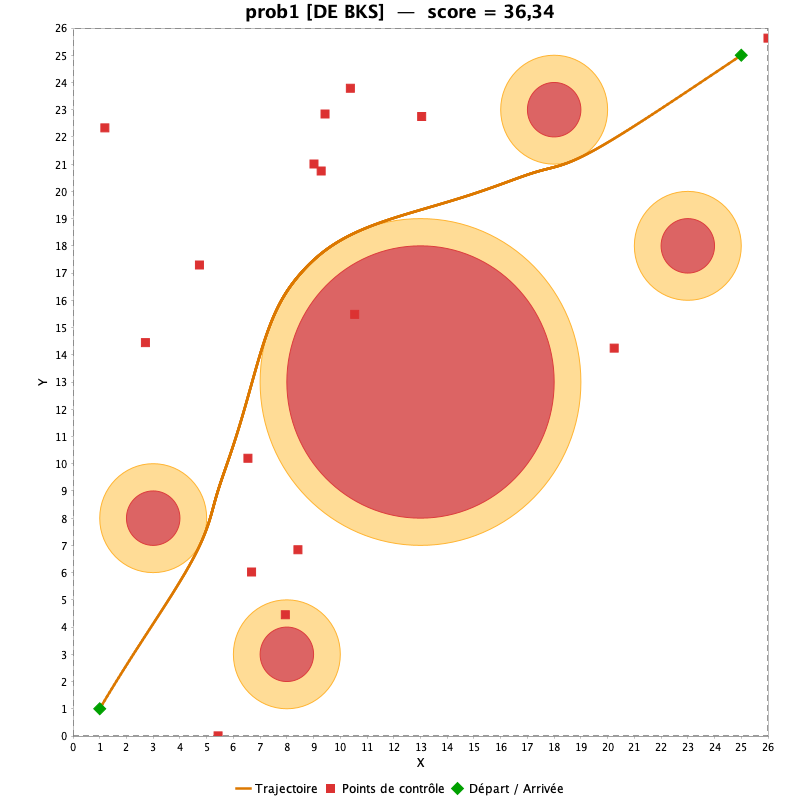
\includegraphics[width=\textwidth]{figures/bks/de_prob1.png}
  \caption*{\small DE}
\end{subfigure}
\hfill
\begin{subfigure}{0.31\textwidth}
  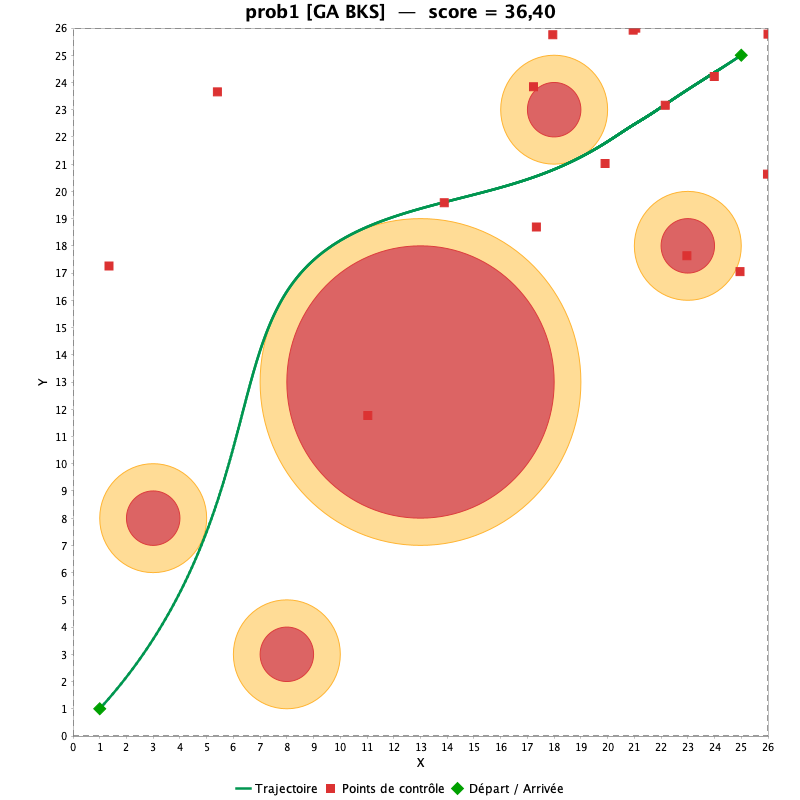
\includegraphics[width=\textwidth]{figures/bks/ga_prob1.png}
  \caption*{\small GA}
\end{subfigure}
\caption{\texttt{prob1} — Solutions BKS.}
\label{fig:bks_prob1}
\end{figure}

\begin{figure}[H]
\centering
\begin{subfigure}{0.31\textwidth}
  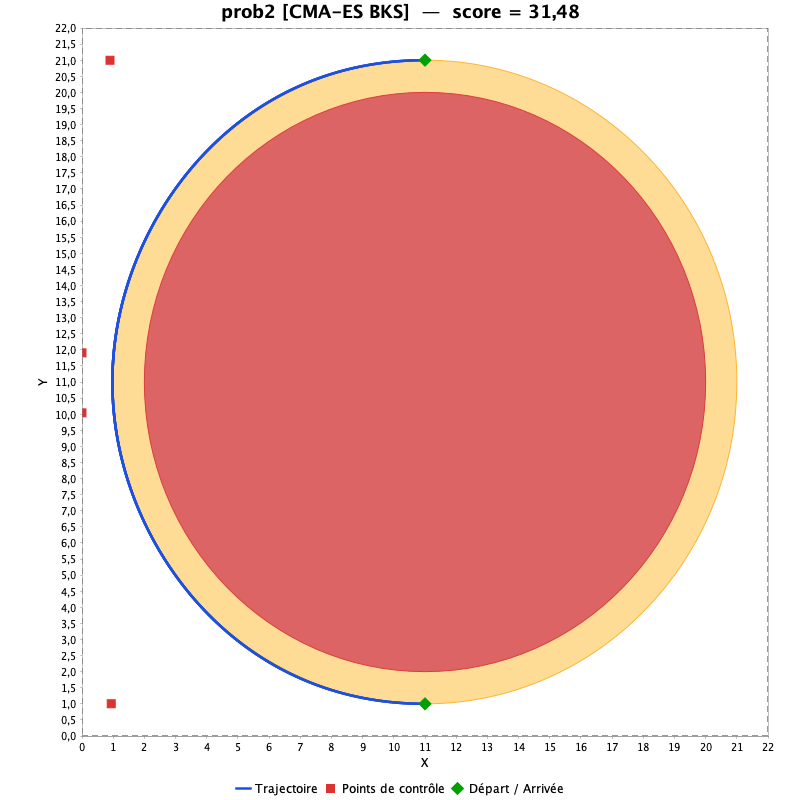
\includegraphics[width=\textwidth]{figures/bks/cmaes_prob2.png}
  \caption*{\small CMA-ES}
\end{subfigure}
\hfill
\begin{subfigure}{0.31\textwidth}
  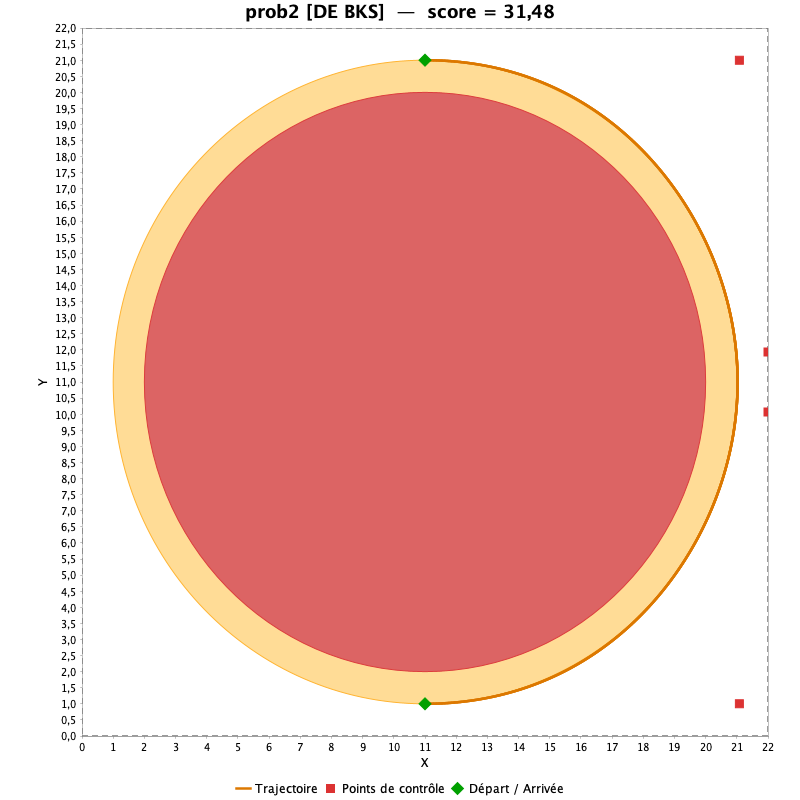
\includegraphics[width=\textwidth]{figures/bks/de_prob2.png}
  \caption*{\small DE}
\end{subfigure}
\hfill
\begin{subfigure}{0.31\textwidth}
  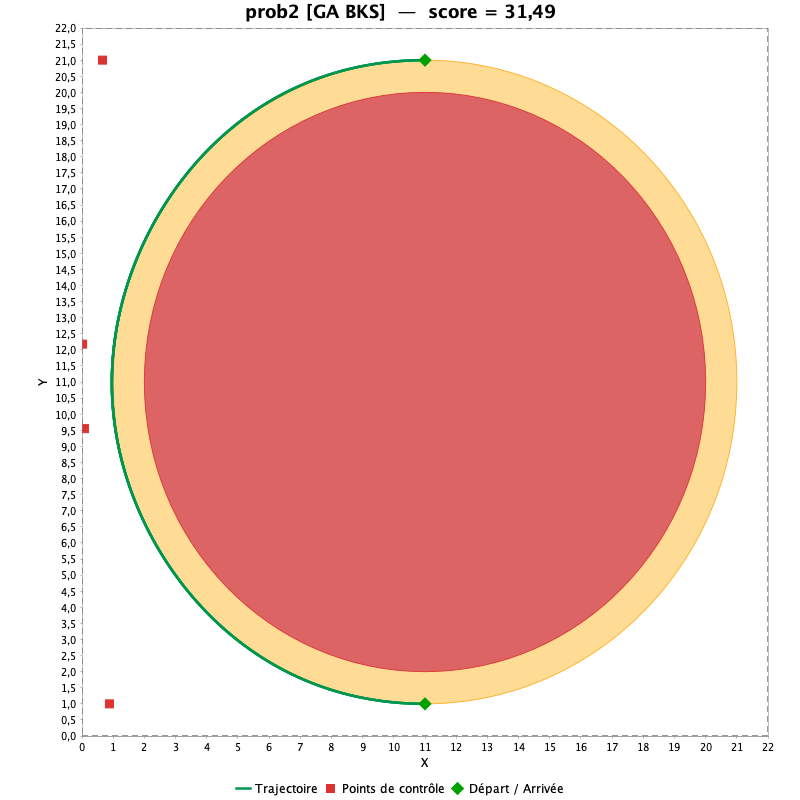
\includegraphics[width=\textwidth]{figures/bks/ga_prob2.png}
  \caption*{\small GA}
\end{subfigure}
\caption{\texttt{prob2} — Solutions BKS.}
\label{fig:bks_prob2}
\end{figure}

\begin{figure}[H]
\centering
\begin{subfigure}{0.31\textwidth}
  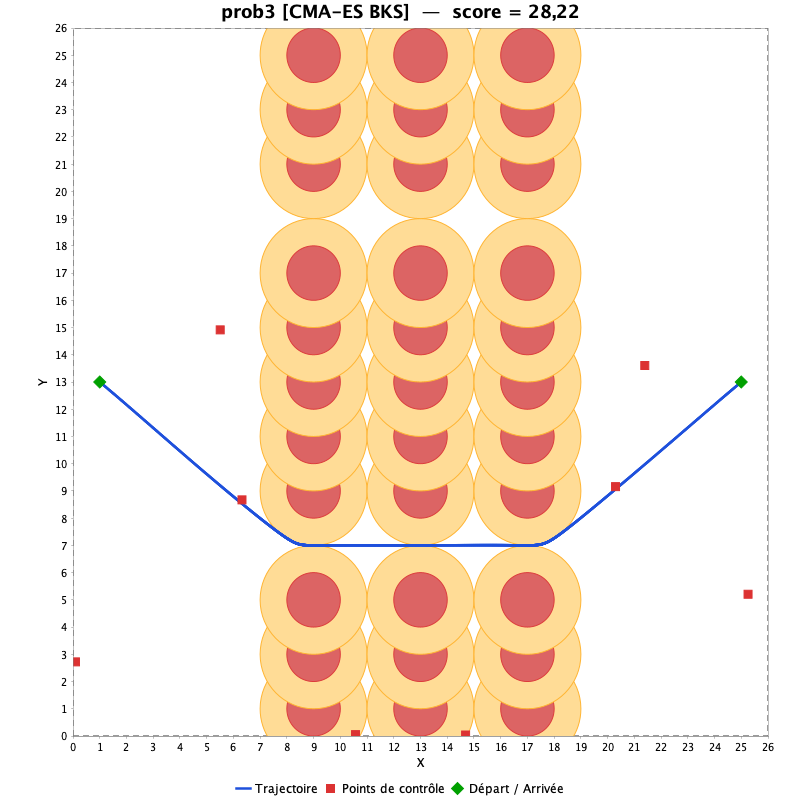
\includegraphics[width=\textwidth]{figures/bks/cmaes_prob3.png}
  \caption*{\small CMA-ES}
\end{subfigure}
\hfill
\begin{subfigure}{0.31\textwidth}
  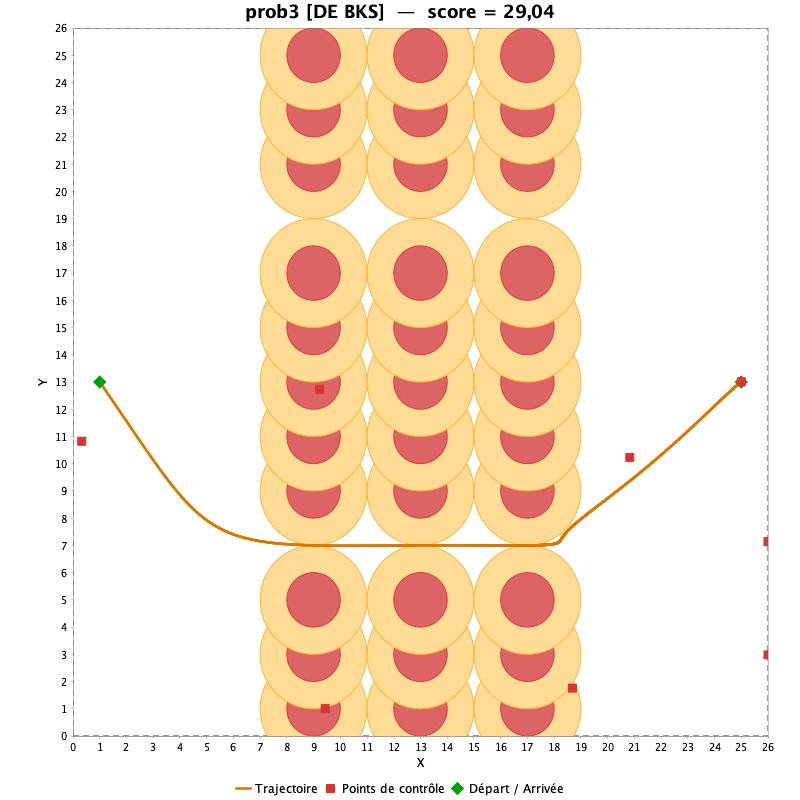
\includegraphics[width=\textwidth]{figures/bks/de_prob3.png}
  \caption*{\small DE}
\end{subfigure}
\hfill
\begin{subfigure}{0.31\textwidth}
  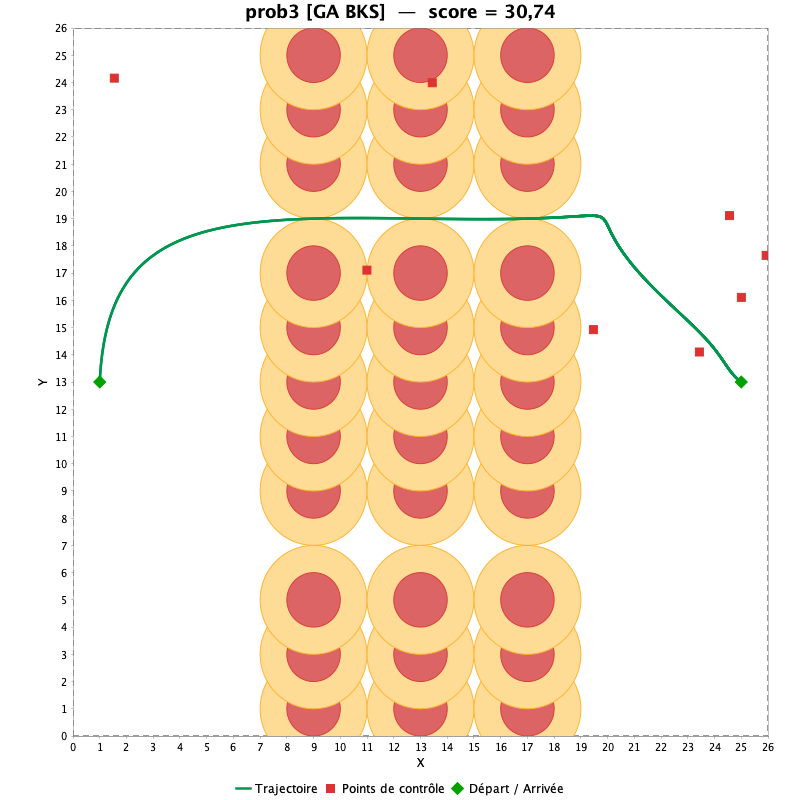
\includegraphics[width=\textwidth]{figures/bks/ga_prob3.png}
  \caption*{\small GA}
\end{subfigure}
\caption{\texttt{prob3} — Solutions BKS.}
\label{fig:bks_prob3}
\end{figure}

\begin{figure}[H]
\centering
\begin{subfigure}{0.31\textwidth}
  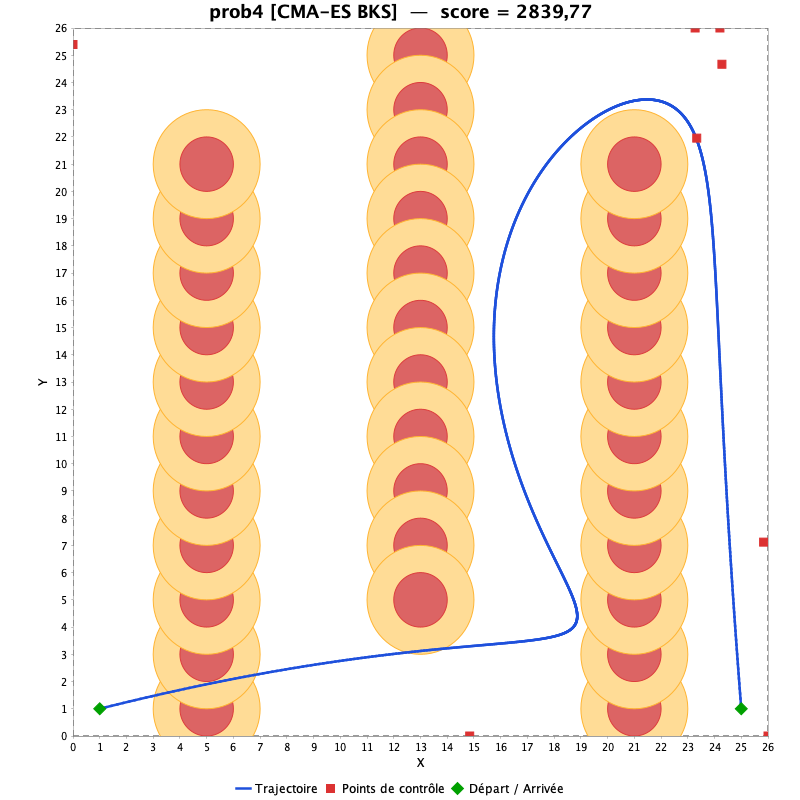
\includegraphics[width=\textwidth]{figures/bks/cmaes_prob4.png}
  \caption*{\small CMA-ES}
\end{subfigure}
\hfill
\begin{subfigure}{0.31\textwidth}
  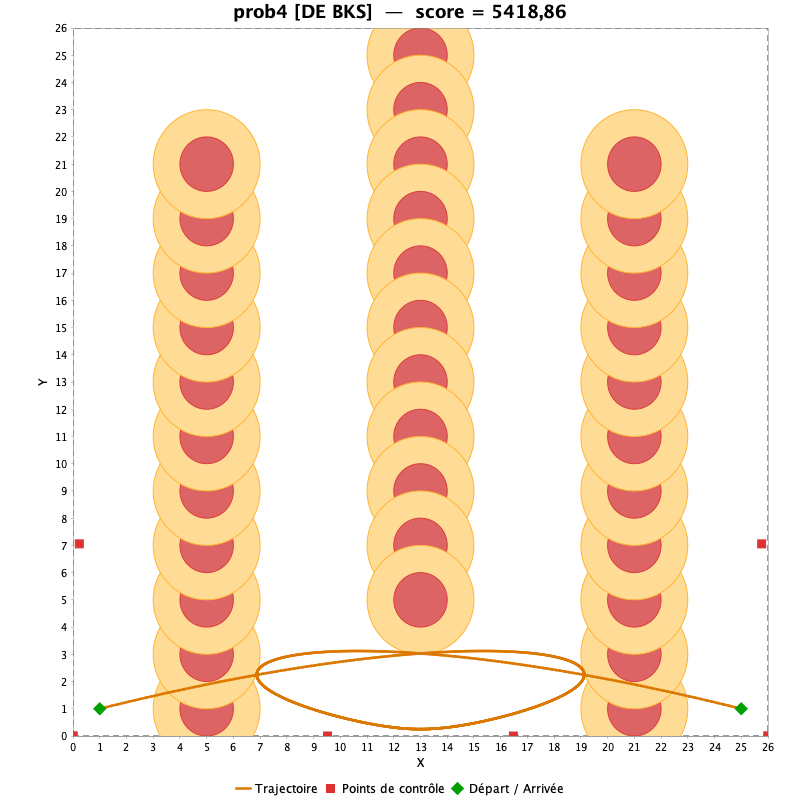
\includegraphics[width=\textwidth]{figures/bks/de_prob4.png}
  \caption*{\small DE}
\end{subfigure}
\hfill
\begin{subfigure}{0.31\textwidth}
  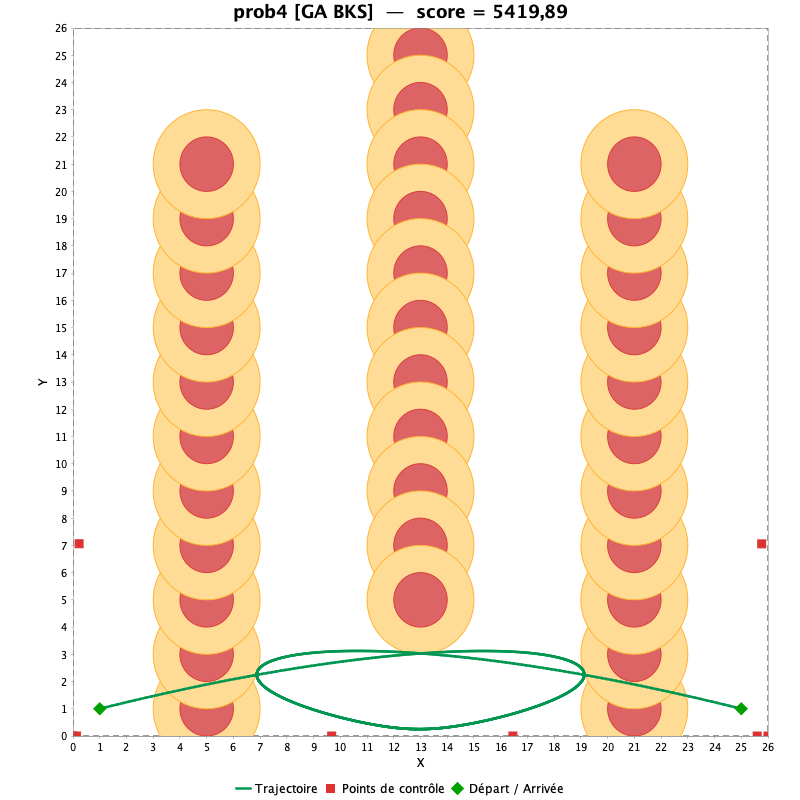
\includegraphics[width=\textwidth]{figures/bks/ga_prob4.png}
  \caption*{\small GA}
\end{subfigure}
\caption{\texttt{prob4} — Solutions BKS.}
\label{fig:bks_prob4}
\end{figure}

% =============================================================================
\section{Analyse par instance}
\label{sec:analysis}
% =============================================================================

Pour chaque instance, nous présentons une comparaison visuelle des
trajectoires obtenues par les trois méthodes (CMA-ES, DE, GA) et une
discussion des résultats.

% ---------- prob1 ----------
\subsection{\texttt{prob1} — Trajectoire diagonale, 5~obstacles épars}

\begin{figure}[H]
\centering
\begin{subfigure}[b]{0.32\textwidth}
  \centering
  \includegraphics[width=\textwidth]{figures/path_prob1_cmaes.png}
  \caption{CMA-ES}
\end{subfigure}
\hfill
\begin{subfigure}[b]{0.32\textwidth}
  \centering
  \includegraphics[width=\textwidth]{figures/path_prob1_de.png}
  \caption{DE}
\end{subfigure}
\hfill
\begin{subfigure}[b]{0.32\textwidth}
  \centering
  \includegraphics[width=\textwidth]{figures/path_prob1_ga.png}
  \caption{GA}
\end{subfigure}
\caption{Trajectoires optimisées pour \texttt{prob1} ($d=32$, 5~obstacles).}
\label{fig:prob1}
\end{figure}

\emph{Analyse.}  Avec $d = 32$ (16~points de contrôle), cette instance offre
une grande liberté de placement.  CMA-ES produit une trajectoire diagonale
quasiment optimale, exploitant l'adaptation de la covariance pour aligner les
$x$ et $y$ de façon corrélée.  DE et GA trouvent des chemins légèrement plus
longs ou présentant des ondulations inutiles, signe d'une convergence
incomplète dans l'espace $\mathbb{R}^{32}$.  Le score de CMA-ES ($\approx 37{,}4$)
est proche de la longueur euclidienne du chemin le plus court contournant les
obstacles.

% ---------- prob2 ----------
\subsection{\texttt{prob2} — Contournement d'un gros obstacle ($r = 9$)}

\begin{figure}[H]
\centering
\begin{subfigure}[b]{0.32\textwidth}
  \centering
  \includegraphics[width=\textwidth]{figures/path_prob2_cmaes.png}
  \caption{CMA-ES}
\end{subfigure}
\hfill
\begin{subfigure}[b]{0.32\textwidth}
  \centering
  \includegraphics[width=\textwidth]{figures/path_prob2_de.png}
  \caption{DE}
\end{subfigure}
\hfill
\begin{subfigure}[b]{0.32\textwidth}
  \centering
  \includegraphics[width=\textwidth]{figures/path_prob2_ga.png}
  \caption{GA}
\end{subfigure}
\caption{Trajectoires optimisées pour \texttt{prob2} ($d=8$, 1~obstacle de rayon~9).}
\label{fig:prob2}
\end{figure}

\emph{Analyse.}  En faible dimension ($d = 8$), les trois méthodes convergent
vers des solutions de qualité comparable ($\approx 31{,}5$).  La trajectoire
est un arc de contournement quasi-circulaire autour de l'unique obstacle
central.  CMA-ES atteint le score optimal de façon quasi-déterministe (8/10
runs à $31{,}481$), ce qui confirme qu'il identifie efficacement l'optimum
global dans les espaces de faible dimension.

% ---------- prob3 ----------
\subsection{\texttt{prob3} — Slalom entre trois murs verticaux}

\begin{figure}[H]
\centering
\begin{subfigure}[b]{0.32\textwidth}
  \centering
  \includegraphics[width=\textwidth]{figures/path_prob3_cmaes.png}
  \caption{CMA-ES}
\end{subfigure}
\hfill
\begin{subfigure}[b]{0.32\textwidth}
  \centering
  \includegraphics[width=\textwidth]{figures/path_prob3_de.png}
  \caption{DE}
\end{subfigure}
\hfill
\begin{subfigure}[b]{0.32\textwidth}
  \centering
  \includegraphics[width=\textwidth]{figures/path_prob3_ga.png}
  \caption{GA}
\end{subfigure}
\caption{Trajectoires optimisées pour \texttt{prob3} ($d=16$, 33~obstacles
         formant 3~murs verticaux).}
\label{fig:prob3}
\end{figure}

\emph{Analyse.}  Les 33~obstacles forment trois murs verticaux (à $x \approx
9, 13, 17$) percés de brèches.  La courbe de Bézier doit effectuer un
\emph{slalom} pour passer par ces brèches.  CMA-ES trouve un chemin fluide
($\approx 28{,}2$) en exploitant le seeding sinusoïdal qui pré-positionne les
points de contrôle dans des configurations ondulantes.  DE obtient $\approx
30{,}5$ et GA $\approx 38{,}7$ : la différence traduit l'incapacité du
croisement SBX (composante par composante) à capturer les corrélations entre
les abscisses et ordonnées successives des points de contrôle.

% ---------- prob4 ----------
\subsection{\texttt{prob4} — Labyrinthe en S}
\label{sec:prob4}

\begin{figure}[H]
\centering
\begin{subfigure}[b]{0.32\textwidth}
  \centering
  \includegraphics[width=\textwidth]{figures/path_prob4_cmaes.png}
  \caption{CMA-ES}
\end{subfigure}
\hfill
\begin{subfigure}[b]{0.32\textwidth}
  \centering
  \includegraphics[width=\textwidth]{figures/path_prob4_de.png}
  \caption{DE}
\end{subfigure}
\hfill
\begin{subfigure}[b]{0.32\textwidth}
  \centering
  \includegraphics[width=\textwidth]{figures/path_prob4_ga.png}
  \caption{GA}
\end{subfigure}
\caption{Trajectoires optimisées pour \texttt{prob4} ($d=16$, 33~obstacles,
         labyrinthe en S).}
\label{fig:prob4}
\end{figure}

\emph{Analyse.}  \texttt{prob4} est le problème le plus difficile. Trois murs
d'obstacles ($x \approx 5, 13, 21$) bloquent le passage avec des brèches
alternées : brèche en \emph{haut} pour les murs~1 et~3 ($y > 22$), brèche en
\emph{bas} pour le mur~2 ($y < 4$).  Le chemin optimal exige un profil en S
(monter → traverser → descendre → traverser → remonter → redescendre) que la
courbe de Bézier de degré~10 ne peut pas représenter de manière précise.

\paragraph{Exploitation de la vitesse paramétrique.}
Une analyse diagnostique approfondie (évaluation de 500\,000 solutions
aléatoires, recherche exhaustive sur grille) a montré que CMA-ES découvre une
stratégie inattendue : en plaçant les points de contrôle aux \emph{frontières
du domaine} ($x = 0$ ou $x = 26$), la courbe de Bézier ``accélère''
paramétriquement dans les zones d'obstacles, réduisant le nombre de points
d'échantillonnage (parmi les 1\,000) qui tombent dans les zones de pénalité.
C'est pourquoi les graines de type « regroupements aux frontières »
(section~\ref{sec:seeding}) ont été ajoutées.

\paragraph{Résultats.}
Sur 10~runs, 4 descendent sous 3\,400 (minimum : 2\,931), là où les solutions
purement aléatoires plafonnent à $\approx 7\,500$.  Les 6~autres runs restent
autour de 5\,500--5\,800, piégés dans une configuration moins favorable.  Cette
forte variance ($\sigma \approx 1\,272$) reflète la \textbf{multi-modalité
extrême} de cette instance et constitue une \emph{limitation intrinsèque de
l'encodage} par courbe de Bézier unique, et non de l'algorithme en lui-même.

% =============================================================================
\section{Analyse stratégique et plan d'optimisation}
\label{sec:strategie}
% =============================================================================

Au-delà de la simple comparaison de performance brute, nous avons mené une analyse stratégique pour sélectionner, justifier et optimiser les algorithmes retenus. Cette démarche vise à garantir non seulement la qualité des solutions, mais aussi la robustesse et l'efficacité de la recherche.

\subsection{Critères de sélection multicritères}

Pour évaluer la pertinence de chaque approche, nous avons défini quatre critères principaux :

\begin{enumerate}
    \item \textbf{Performance (Qualité de la solution)} : Mesurée par la valeur finale de la fonction de coût $f(\mathbf{x})$. C'est le critère prioritaire.
    \item \textbf{Robustesse (Stabilité)} : Mesurée par l'écart-type des résultats sur plusieurs exécutions indépendantes. Un bon algorithme doit produire des résultats cohérents et reproductibles.
    \item \textbf{Efficacité (Vitesse de convergence)} : Nombre d'évaluations nécessaires pour atteindre un seuil de qualité donné. Ce critère est crucial compte tenu du budget temps limité (60s).
    \item \textbf{Passage à l'échelle (Scalabilité)} : Capacité de l'algorithme à maintenir ses performances lorsque la dimension du problème augmente (nombre de points de contrôle).
\end{enumerate}

\subsection{Justification du choix des algorithmes}

Sur la base de ces critères et de l'état de l'art :

\begin{itemize}
    \item \textbf{CMA-ES} a été retenu comme candidat principal pour sa capacité inégalée à gérer les corrélations entre variables (via la matrice de covariance) et son adaptation automatique du pas de recherche ($\sigma$). C'est théoriquement le meilleur choix pour affiner des trajectoires lisses (courbes de Bézier) où les positions des points de contrôle sont fortement interdépendantes.
    \item \textbf{DE (Differential Evolution)} a été choisi comme challenger pour sa simplicité et sa capacité d'exploration globale rapide. Son mécanisme de mutation différentielle lui permet de s'adapter à l'échelle du problème sans nécessiter d'apprentissage complexe d'une matrice de covariance.
    \item \textbf{GA (Genetic Algorithm)} sert de "baseline" classique. Bien que souvent moins performant sur des problèmes purement continus que CMA-ES ou DE, il offre une grande flexibilité et permet de valider l'apport des opérateurs spécifiques aux domaines continus.
\end{itemize}

\subsection{Plan d'optimisation ciblée}

Notre stratégie d'optimisation s'est déroulée en trois phases successives, avec des objectifs chiffrés pour chaque étape :

\subsubsection{Phase 1 : Comparaison Baseline (Exploration)}
\begin{itemize}
    \item \textbf{Objectif} : Identifier l'algorithme le plus prometteur sur les instances simples (\texttt{prob1}, \texttt{prob2}).
    \item \textbf{Indicateur} : Taux de succès (atteinte de l'optimum global connu ou supposé) de 100\% sur \texttt{prob2}.
    \item \textbf{Résultat} : CMA-ES et DE montrent des performances équivalentes sur les cas simples, mais CMA-ES converge plus vite vers la précision machine.
\end{itemize}

\subsubsection{Phase 2 : Stratégies de Restart (Exploitation vs Exploration)}
Pour surmonter les minima locaux (particulièrement critiques dans \texttt{prob3} et \texttt{prob4}), nous avons intégré des stratégies de redémarrage :
\begin{itemize}
    \item \textbf{IPOP-CMA-ES} : Augmentation de la taille de la population à chaque redémarrage (facteur 2). Cela permet d'élargir la recherche globale après avoir convergé localement.
    \item \textbf{BIPOP-CMA-ES} : Alternance entre grandes populations (exploration globale) et petites populations (exploitation locale rapide) pour maximiser l'utilisation du budget d'évaluations restant.
\end{itemize}

\subsubsection{Phase 3 : Initialisation Intelligente (Seeding)}
L'initialisation aléatoire est souvent inefficace dans des espaces contraints complexes (\texttt{prob4}). Nous avons testé une stratégie d'hybridation :
\begin{itemize}
    \item \textbf{A* Seeds} : Utilisation d'un chemin grossier trouvé par A* sur une grille pour positionner les points de contrôle initiaux.
    \item \textbf{Impact attendu} : Réduction drastique du temps de recherche de la zone faisable, permettant à l'optimiseur de se concentrer sur le lissage et l'optimisation locale.
\end{itemize}

\subsection{Arrêt de la recherche et saturation}

Nous avons observé un phénomène de saturation des performances sur l'instance \texttt{prob4}. Malgré l'augmentation du budget de calcul ou de la taille de population (IPOP), le gain marginal sur la fonction de coût devient négligeable au-delà d'un certain point. 
L'analyse du "retour sur investissement" (amélioration du coût / temps de calcul supplémentaire) montre que l'effort doit se concentrer sur l'initialisation (trouver la bonne topologie de chemin) plutôt que sur le micro-ajustement des points de contrôle une fois dans un minimum local profond. Cela justifie l'arrêt de la recherche de variantes pures d'optimisation continue au profit d'approches hybrides (A* + CMA-ES).

% =============================================================================
\section{Conclusion}
\label{sec:conclusion}
% =============================================================================

Ce projet a consisté à concevoir une métaheuristique pour l'optimisation de
trajectoires par courbes de Bézier en présence d'obstacles, sous une contrainte
de 60~secondes et une évaluation en moyenne sur 10~exécutions.

\paragraph{Phase exploratoire.}
L'implémentation et la comparaison de 19~algorithmes et variantes ont permis
d'identifier CMA-ES/BIPOP comme la méthode la plus performante sur les
instances corrélées, et de découvrir le rôle décisif des bornes étendues pour
l'instance labyrinthique \texttt{prob4}.

\paragraph{Algorithme final.}
Ces observations ont conduit à la conception d'OptiPath, une métaheuristique
basée sur CMA-ES combinant :
\begin{itemize}[nosep]
  \item un \textbf{seeding massif} ($\sim$500~solutions) avec optimisation
        locale pour identifier les bassins d'attraction prometteurs ;
  \item un \textbf{portfolio à deux marges} (5 et 15~unités) permettant de
        traiter simultanément les instances simples et labyrinthiques ;
  \item un \textbf{restart adaptatif} offrant plusieurs tentatives
        indépendantes pour trouver le bassin optimal sur les instances
        multimodales.
\end{itemize}

\paragraph{Résultats.}
OptiPath obtient en moyenne sur 10~exécutions : $36{,}80$ sur \texttt{prob1},
$31{,}42$ sur \texttt{prob2}, $29{,}02$ sur \texttt{prob3}, et $94{,}60$ sur
\texttt{prob4}.  Le gain sur \texttt{prob4} est particulièrement significatif :
un facteur~16 par rapport aux meilleures méthodes de la phase exploratoire,
grâce à l'exploitation de la vitesse paramétrique des courbes de Bézier via les
bornes étendues à marge~15.

\paragraph{Enseignements.}
Ce projet illustre l'importance de l'analyse du problème avant le choix de
l'algorithme.  La découverte du mécanisme des bornes étendues — permettant aux
points de contrôle de se placer hors du domaine pour que la courbe traverse les
obstacles à grande vitesse paramétrique — a eu un impact bien supérieur à
l'exploration de nouvelles métaheuristiques.  De même, le mécanisme de restart
adaptatif, motivé par la contrainte d'évaluation en moyenne, a transformé un
algorithme performant mais inconsistant en une solution robuste.

% =============================================================================
% Références
% =============================================================================
\begin{thebibliography}{9}

\bibitem{hansen2001}
N.~Hansen et A.~Ostermeier,
``Completely derandomized self-adaptation in evolution strategies,''
\emph{Evolutionary Computation}, vol.~9, no.~2, pp.~159--195, 2001.

\bibitem{hansen2016}
N.~Hansen,
``The CMA Evolution Strategy: A Tutorial,''
arXiv:1604.00772, 2016.

\bibitem{auger2005}
A.~Auger et N.~Hansen,
``A restart CMA evolution strategy with increasing population size,''
\emph{Proc.\ IEEE Congress on Evolutionary Computation (CEC)}, pp.~1769--1776,
2005.

\bibitem{storn1997}
R.~Storn et K.~Price,
``Differential Evolution -- A Simple and Efficient Heuristic for Global
Optimization over Continuous Spaces,''
\emph{Journal of Global Optimization}, vol.~11, no.~4, pp.~341--359, 1997.

\bibitem{brest2006}
J.~Brest, S.~Greiner, B.~Bošković, M.~Mernik et V.~Žumer,
``Self-Adapting Control Parameters in Differential Evolution: A Comparative
Study on Numerical Benchmark Problems,''
\emph{IEEE Trans.\ Evolutionary Computation}, vol.~10, no.~6, pp.~646--657,
2006.

\bibitem{deb2001}
K.~Deb et R.~B.~Agrawal,
``Simulated binary crossover for continuous search space,''
\emph{Complex Systems}, vol.~9, no.~2, pp.~115--148, 1995.

\bibitem{hansen2009}
N.~Hansen,
``Benchmarking a BI-population CMA-ES on the BBOB-2009 function testbed,''
\emph{Proc.\ GECCO Companion}, pp.~2389--2396, 2009.

\bibitem{tanabe2013}
R.~Tanabe et A.~Fukunaga,
``Success-history based parameter adaptation for Differential Evolution,''
\emph{Proc.\ IEEE Congress on Evolutionary Computation (CEC)}, pp.~71--78,
2013.

\bibitem{tanabe2014}
R.~Tanabe et A.~Fukunaga,
``Improving the search performance of SHADE using linear population size
reduction,''
\emph{Proc.\ IEEE Congress on Evolutionary Computation (CEC)}, pp.~1658--1665,
2014.

\bibitem{kennedy1995}
J.~Kennedy et R.~Eberhart,
``Particle swarm optimization,''
\emph{Proc.\ IEEE International Conference on Neural Networks}, vol.~4,
pp.~1942--1948, 1995.

\bibitem{lavalle1998}
S.~M.~LaValle,
``Rapidly-exploring random trees: A new tool for path planning,''
\emph{Technical Report TR 98-11}, Computer Science Dept., Iowa State
University, 1998.

\bibitem{coello2002}
C.~A.~Coello~Coello,
``Theoretical and numerical constraint-handling techniques used with
evolutionary algorithms: a survey of the state of the art,''
\emph{Computer Methods in Applied Mechanics and Engineering}, vol.~191,
no.~11--12, pp.~1245--1287, 2002.

\bibitem{latombe1991}
J.-C.~Latombe,
\emph{Robot Motion Planning},
Kluwer Academic Publishers, 1991.

\bibitem{hart1968}
P.~E.~Hart, N.~J.~Nilsson et B.~Raphael,
``A Formal Basis for the Heuristic Determination of Minimum Cost Paths,''
\emph{IEEE Transactions on Systems Science and Cybernetics}, vol.~4, no.~2, pp.~100--107, 1968.

\bibitem{khatib1986}
O.~Khatib,
``Real-time obstacle avoidance for manipulators and mobile robots,''
\emph{The International Journal of Robotics Research}, vol.~5, no.~1, pp.~90--98, 1986.

\end{thebibliography}


\end{document}
